\documentclass[11pt, twocolumn]{article}

\usepackage[spanish]{babel}
\usepackage[none]{hyphenat}
\usepackage[left=1.2cm, right=1.2cm, top = 2cm, bottom=2.5cm]{geometry}
% \usepackage{setspace}
\usepackage{parskip}
\usepackage[export]{adjustbox}
\usepackage{enumitem}
\usepackage{listings}
\usepackage[dvipsnames]{xcolor}
\usepackage{fancyhdr}
\usepackage{graphicx}
\usepackage{caption}
% \usepackage{subcaption}
% \usepackage{wrapfig}
% \usepackage{multirow, makecell}
% \usepackage{float}
% \usepackage{amsmath} 
% \usepackage{amsfonts}
\usepackage[hidelinks]{hyperref}
\usepackage{csquotes}

\newcommand{\linejump}{\hfill \break}
\renewcommand{\thefootnote}{\fnsymbol{footnote}}
% \newcommand{\unit}[1]{\ensuremath{\, \mathrm{#1}}}

\definecolor{dkgreen}{rgb}{0,0.6,0}
\definecolor{gray}{rgb}{0.5,0.5,0.5}
\definecolor{mauve}{rgb}{0.58,0,0.82}
\lstset{
  language=Java,
  aboveskip=3mm,
  belowskip=3mm,
  showstringspaces=false,
  columns=flexible,
  basicstyle={\tiny\ttfamily},
  numbers=none,
  numberstyle=\tiny\color{gray},
  keywordstyle=\color{blue},
  commentstyle=\color{dkgreen},
  stringstyle=\color{mauve},
  breaklines=true,
  breakatwhitespace=true,
  tabsize=2
}

\sloppy
\setlength{\parindent}{0cm}
\setlength{\columnsep}{0.5cm}
\decimalpoint
\graphicspath{{img/}}

\hypersetup{colorlinks=true, urlcolor=blue, citecolor=blue}
\urlstyle{same}

\pagestyle{fancyplain}
\fancyhf{}
\fancyhead[L]{\scriptsize 
  Universidad Nacional Autónoma de México \\
  Laboratorio de Programación Orientada a Objetos \\
  M.C. Leonardo Ledesma Dominguez
}
\fancyhead[R]{\thepage}

\begin{document}
  \twocolumn[
    \centering
    Acosta Porcayo Alan Omar, Gutiérrez Grimaldo Alejandro, Medina Villa Samuel

    \linejump

    \textbf{\LARGE{Práctica 12. Hilos}} \\
    
    \linejump
  ]
      
  \footnotetext{
    \scriptsize 
    Acosta Porcayo Alan Omar Ing. en Computación 320206102 \\
    Gutiérrez Grimaldo Alejandro Ing. en Computación 320282098 \\
    Medina Villa Samuel Ing. en Computación 320249538
  }
        
  \fancyfoot{}

  \section*{Resumen}
  La práctica se enfoca en la implementación del concepto de multitarea mediante hilos en un entorno orientado a objetos. Se abordarán dos enfoques principales: la creación de hilos con la clase \textit{Thread} y la interfaz \textit{Runnable}. La práctica incluirá ejercicios prácticos para aplicar estos conceptos, evaluación de ventajas y desventajas entre ambos enfoques, y la exploración de la ejecución concurrente de tareas, haciendo hincapié en la coordinación efectiva de hilos para mejorar la eficiencia en programas concurrentes.

  \section*{Introducción}
  Imaginemos el desafío de desarrollar una aplicación departamental encargada de realizar diversas operaciones complejas. Entre estas funciones críticas se encuentran la descarga del catálogo de precios de productos recién incorporados al inventario, la realización de la contabilidad correspondiente al día anterior y la aplicación de descuentos a productos ya existentes en el sistema.

  \subsection*{Inconvenientes de la Ejecución Secuencial}
  En un flujo de ejecución convencional, estas tareas se llevarían a cabo de manera secuencial, una después de la otra. No obstante, la ejecución secuencial plantea inconvenientes, especialmente cuando la descarga de productos nuevos consume demasiado tiempo, afectando la aplicación oportuna de descuentos. En este escenario, la eficiencia se ve comprometida, y la respuesta a solicitudes específicas, como productos con descuentos, se ve demorada.

  \subsection*{Solución Ideal: Hilos (\textit{Threads})}
  La solución ideal radica en la implementación de varios flujos de ejecución simultánea para que una tarea no dependa de la finalización de otras. La herramienta fundamental para lograr esto son los hilos, donde cada hilo representa una tarea independiente.

  \subsection*{Exploración de Hilos en Java}
  En este contexto, exploramos el concepto de hilos (\textit{threads}), que son flujos de ejecución individuales dentro de un proceso. En Java, la Máquina Virtual (JVM) tiene la capacidad de manejar multihilos, permitiendo la creación de varios flujos de ejecución simultánea. Esto se gestiona a través de clases y una interfaz específicas, como \textit{Thread} y \textit{Runnable}.

  \subsection*{Ciclo de Vida de un Hilo}
  La práctica se enfocará en comprender y aplicar el ciclo de vida de un hilo, desde su estado inicial hasta su finalización. Se destacan características importantes, como los estados \textit{``new''}, \textit{``runnable''}, \textit{``not running''} y \textit{``dead''} y se explora cómo los hilos pueden regresar al estado \textit{``runnable''} según la situación.

  \subsection*{Planificador (\textit{Scheduler}) y Prioridad}
  Exploramos el papel crucial del planificador (\textit{Scheduler}) de Java, que decide qué hilos deben ejecutarse según su prioridad. La prioridad de un hilo, modificable a lo largo de su vida, determina su orden de ejecución.

  \subsection*{Clases y Elementos Clave}
  Adicionalmente, se abordan las clases \textit{Thread}, \textit{Runnable}, \textit{ThreadDeath}, y \textit{ThreadGroup}, proporcionando una visión integral de cómo Java gestiona los hilos. Características importantes incluyen el método run que define la acción de un hilo, los métodos \textit{start} y stop para iniciar y detener la ejecución del hilo, y la capacidad de agrupar hilos mediante \textit{ThreadGroup}.

  \subsection*{Métodos o Bloques Sincronizados}
  También se explora la importancia de los métodos o bloques sincronizados para evitar conflictos de acceso en entornos de ejecución paralela. Estos aseguran que solo un hilo acceda a un método sincronizado al mismo tiempo, evitando pérdida de información.

  \section*{Objetivos}
  \begin{itemize}
    \item Implementar hilos utilizando la clase \textit{Thread}. 
    \item Implementar hilos utilizando la interfaz \textit{Runnable}.
    \item Desarrollar habilidades para gestionar excepciones específicas de hilos.
  \end{itemize}

  \section*{Metodología}
  \textit{\textbf{Hilo.java}}
  \begin{lstlisting}
public class Hilo extends Thread{
	public Hilo(String nombre){
		super(nombre);
	}
	public void run(){
		for(int i= 0; i<5; i++){
			System.out.println("iteracion: " + (i+1) + "de" + getName());
		}
		System.out.println("Termina el " + getName());

	}

	public static void main(String[] args) {
		new Hilo ("Primer hilo").start();
		new Hilo ("Segundo hilo").start();
		System.out.println("Termina el hilo principal");
		
	}
}
  \end{lstlisting}

  \textit{\textbf{Cuenta.java}}
  \begin{lstlisting}
class Cuenta extends Thread{
	private static long saldo = 0;
	public Cuenta(String nombre){
		super(nombre);

	}

	public void run(){
		if (getName().equals("Deposito 1") || getName().equals("Deposito 2")){
			this.depositarDinero(100);
		}else{
			this.extraerDinero(50);
		}
	}

	public synchronized void extraerDinero(int cantidad){
		try{

			if(saldo <= 0){
				System.out.println(getName() + "espera a que depositen lana");
				sleep(5000);

			}

		}catch(InterruptedException e){
			System.out.println(e);

		}

		saldo-= cantidad;
		System.out.println(getName() + "extrajo 50, el saldo es: " + saldo);
		notifyAll();

	}

	public synchronized void depositarDinero(int cantidad){
		saldo += cantidad;
		System.out.println("Se deposito dinero (100), el saldo es: " + saldo );
		notifyAll();

	}
	public static void main(String[] args) {
		new Cuenta("Acceso A").start();
		new Cuenta("Acceso B").start();
		new Cuenta("Deposito 1 ").start();
		new Cuenta("Deposito 2 ").start();
		System.out.println("termina el main");
	}
}
  \end{lstlisting}

  \textit{\textbf{Grupo.java}}
  \begin{lstlisting}
public class Grupo extends Thread{
	public Grupo(ThreadGroup G, String n){
		super(G,n);

	}
	public void run(){
		for (int i=0;i<10 ;i++ ) {
			System.out.println(getName());
			
		}
	}

	public static void listarHilos(ThreadGroup grupoActual){
		int numhilos;
		Thread[]listaHilos;

		numhilos = grupoActual.activeCount();
		listaHilos = new Thread[numhilos];
		System.out.println("Numero de hilos activos en el grupo " + numhilos);
		for (int i=0; i<numhilos ;i++ ) {
			System.out.println("Hilo Activo: " + (i+1) + "=" + listaHilos[i].getName());
			
		}
	
	}

	public static void main(String[] args) {

		ThreadGroup grupoH = new ThreadGroup("Grupo de Hilos prioridad normal");
		Thread hilo1 = new Grupo(grupoH, "Hilo 1 con prioridad normal");
		Thread hilo2 = new Grupo(grupoH, "Hilo 2 con prioridad normal");
		Thread hilo3 = new Grupo(grupoH, "Hilo 3 con prioridad normal");
		Thread hilo4 = new Grupo(grupoH, "Hilo 4 con prioridad normal");
		Thread hilo5 = new Grupo(grupoH, "Hilo 5 con prioridad normal");
		Thread hilo6 = new Grupo(grupoH, "Hilo 6 con prioridad normal");
		Thread hilo7 = new Grupo(grupoH, "Hilo 7 con prioridad normal");
		Thread hilo8 = new Grupo(grupoH, "Hilo 8 con prioridad normal");
		Thread hilo9 = new Grupo(grupoH, "Hilo 9 con prioridad normal");
		Thread hilo10 = new Grupo(grupoH, "Hilo 10 con prioridad normal");

		hilo7.setPriority(Thread.MAX_PRIORITY);
		hilo10.setPriority(Thread.MIN_PRIORITY);
		grupoH.setMaxPriority(Thread.NORM_PRIORITY);

		System.out.println("La prioridad del grupo es de : " + grupoH.getMaxPriority());

		System.out.println("La prioridad del Thread es de : " + hilo1.getPriority());
		System.out.println("La prioridad del Thread es de : " + hilo2.getPriority());
		System.out.println("La prioridad del Thread es de : " + hilo3.getPriority());
		System.out.println("La prioridad del Thread es de : " + hilo4.getPriority());
		System.out.println("La prioridad del Thread es de : " + hilo5.getPriority());
		System.out.println("La prioridad del Thread es de : " + hilo6.getPriority());
		System.out.println("La prioridad del Thread es de : " + hilo7.getPriority());
		System.out.println("La prioridad del Thread es de : " + hilo8.getPriority());
		System.out.println("La prioridad del Thread es de : " + hilo9.getPriority());
		System.out.println("La prioridad del Thread es de : " + hilo10.getPriority());

		hilo1.start();
		hilo2.start();
		hilo3.start();
		hilo4.start();
		hilo5.start();
		hilo6.start();
		hilo7.start();
		hilo8.start();
		hilo9.start();
		hilo10.start();

		listarHilos(grupoH);		
	}	
}
  \end{lstlisting}

  \section*{Resultados}
  \subsection*{Problema 1}
  Modificar el juego de la liebre y la tortuga de la práctica 3 para simular la carrera de manera asíncrona.

  \textit{\textbf{Usar métodos propios de la clase Thread start(), join() y yield()}}

  \textit{\textbf{Solución}}
  \begin{lstlisting}
import java.util.Random;

public class Problema1 {
  static final int N = 10;
  static StringBuilder[][] pista = new StringBuilder[N][N];
  static final int ESPERA = 2000;

  class Corredor extends Thread {
    int pos, i, j;
    final char SIMBOLO;

    Corredor(int pos, int i, int j, char SIMBOLO, String nombre) {
      this.pos = pos;
      this.i = i;
      this.j = j;
      this.SIMBOLO = SIMBOLO;
      setName(nombre);
    }

    @Override
    public void run() {
      synchronized (pista) {
        System.out.println("\nTurno de " + getName() + "\tPosicion: " + pos);
        pos = jugada(pos);
        if (pista[i][j].charAt(pista[i][j].length() - 1) == SIMBOLO)
          pista[i][j].deleteCharAt(pista[i][j].length() - 1);
        else
          pista[i][j].deleteCharAt(pista[i][j].length() - 2);

        if (pos == 0) {
          i = 0;
          j = 0;
        } else {
          i = (pos - 1) / 10;
          j = (pos - 1) % 10;
        }

        pista[i][j].append(SIMBOLO);
        imprimirPista();
        System.out.println("Fin del turno");
        
        try {
          Thread.sleep(ESPERA);
        } catch (InterruptedException e) {
          System.out.println(e);
        } finally {
          Thread.yield();
        }
      }
    }
  }

  static void inicializarPista() {
    int numeroCasilla = 2;

    pista[0][0] = new StringBuilder("S");
    pista[9][9] = new StringBuilder("E");

    for (int i = 0; i < N; i++) {
      for (int j = 0; j < N; j++) {
        if ((i == 0 && j == 0) || (i == 9 && j == 9)) continue;
        else pista[i][j] = new StringBuilder(Integer.toString(numeroCasilla++));
      }
    }

    pista[0][0].append("HT");
  }

  static void imprimirPista() {
    for (int i = 0; i < N; i++) {
      for (int j = 0; j < N; j++)
        System.out.print(pista[i][j] + "\t");
      System.out.println();
    }
  }

  static int jugada(int posActual) {
    Random rand = new Random();
    int dado, posNueva = posActual;

    dado = rand.nextInt(6) + 1;
    posNueva += dado;

    if (posNueva > 100) posNueva = 100;

    System.out.println("Dado: " + dado);
    System.out.println("Avanza de " + posActual + " a " + posNueva);

    switch (posNueva) {
      case 7, 14, 33, 77, 89 -> {
        System.out.println("Casilla Especial!\tTira de nuevo");
        posNueva = jugada(posNueva);
      } case 6, 23, 42, 56, 82, 90 -> {
        System.out.println("Trampa\tRetrocede de " + posNueva + " a " + (posNueva - 5));
        posNueva -= 5;
      } case 36 -> {
        System.out.println("Casilla Especial!\tAvanza de " + posNueva + " a 71");
        posNueva = 71;
      } case 65 -> {
        System.out.println("Casilla Especial!\ttAvanza de " + posNueva + " a 84");
        posNueva = 84;
      } case 10 -> {
        System.out.println("Trampa\tRegresa al inicio");
        posNueva = 1;
      } case 66 -> {
        System.out.println("Trampa\tRegresa de " + posNueva + " a 40");
        posNueva = 40;
      }
    }

    return posNueva;
  }

  public static void main(String[] args) throws InterruptedException {
    int turno = 0;
    Corredor tortuga = new Problema1().new Corredor(1, 0, 0, 'T', "Tortuga");
    Corredor liebre = new Problema1().new Corredor(1, 0, 0, 'H', "Liebre ");

    inicializarPista();

    System.out.println("Pista inicial");
    imprimirPista();
    
    tortuga.start();
    liebre.start();
    Thread.sleep(ESPERA);
    
    while (true) {
      turno++;
      tortuga.join();
      liebre.join();
      tortuga.run();
      Thread.yield();
      liebre.run();
      if (liebre.pos == 100 || tortuga.pos == 100) break;   
    }

    System.out.println("\nGanador: " + (turno % 2 != 0 ? "Tortuga!" : "Liebre!"));
    System.out.println("Fin del juego");
  }
}
  \end{lstlisting}

  \newpage
  \textbf{Ejecución}
  \begin{figure}[h!]
    \centering
    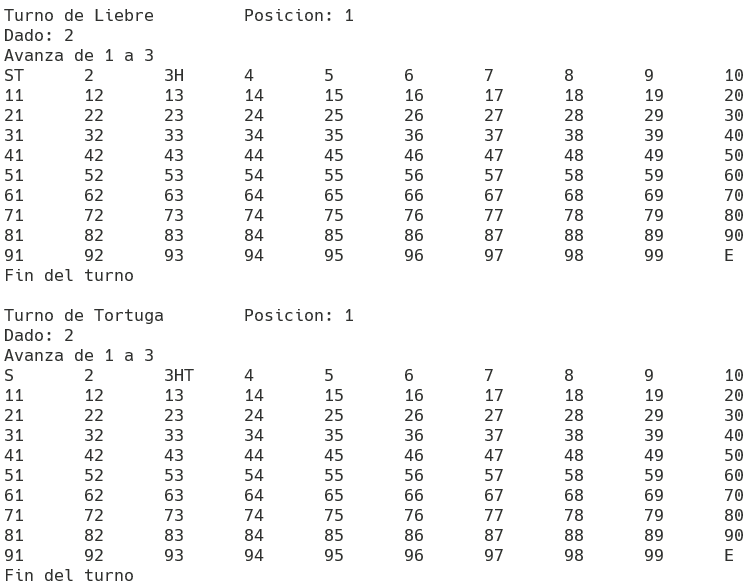
\includegraphics[width=\columnwidth]{12P1.png}
  \end{figure}

  \subsection*{Problema 2}
  Realice un programa que funcione de manera síncrona que simule la interacción de una clase. Primeramente, que cuando un alumno o el profesor entre a clase muestre un letrero ``ingreso a la clase''.

  Y que cuando un profesor (hilo) diga “buenos días”, los alumnos en clase (mínimo 5 hilos) respondan buenos días.

  \textit{\textbf{Usar métodos propios de la clase Thread start(), join(), nofifyAll() y wait()}}

  \textit{\textbf{Solución}}
  \begin{lstlisting}
class Clase {
    public synchronized void entrarClase(String persona) {
      System.out.println(persona + " ingreso a la clase");
    }

    public synchronized void decirBuenosDias() throws InterruptedException {
      System.out.println("Profesor: Buenos dias");
      notifyAll();
    }
}

class Alumno extends Thread {
  private Clase clase;
  private String nombre;

  public Alumno(Clase clase, String nombre) {
    this.clase = clase;
    this.nombre = nombre;
  }

  @Override
  public void run() {
    clase.entrarClase(nombre);
    try {
      synchronized (clase) {
        clase.wait();
        System.out.println(nombre + ": Buenos dias");
      }
    } catch (InterruptedException e) {
      e.printStackTrace();
    }
  }
}

class Profesor extends Thread {
  private Clase clase;

  public Profesor(Clase clase) {
    this.clase = clase;
  }

  @Override
  public void run() {
    clase.entrarClase("Profesor");
    try {
      Thread.sleep(1000);
      clase.decirBuenosDias();
    } catch (InterruptedException e) {
      e.printStackTrace();
    }
  }
}

public class Problema2 {
  public static void main(String[] args) {
    Clase clase = new Clase();

    Profesor profesor = new Profesor(clase);
    profesor.start();

    Alumno[] alumnos = new Alumno[5];
    for (int i = 0; i < alumnos.length; i++) {
      alumnos[i] = new Alumno(clase, "Alumno " + (i + 1));
      alumnos[i].start();
    }

    try {
      profesor.join();
      for (Alumno alumno : alumnos) {
        alumno.join();
      }
    } catch (InterruptedException e) {
      e.printStackTrace();
    }
  }
}
  \end{lstlisting}

  \textbf{Ejecución}
  \begin{figure}[h!]
    \centering
    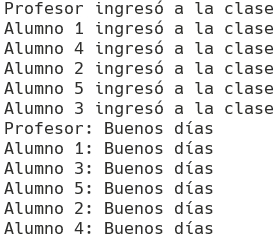
\includegraphics[width=0.5\columnwidth]{12P2.png}
  \end{figure}

  \subsection*{Problema 3}
  Usando variables volátiles y métodos sincronizados programe dos hilos en java que calculen $n$ coeficientes de la secuencia de Ulam en la práctica 5. 

  \textit{\textbf{Usar métodos propios de la interfaz runnable}}

  \textit{\textbf{Solución}}
  \begin{lstlisting}
import java.util.ArrayList;
import java.util.Comparator;
import java.util.Scanner;

class Ulam implements Runnable {
  private static final ArrayList<Integer> sequence = new ArrayList<>();
  private final int u;
  private final int v;
  private final int n;

  public Ulam(int u, int v, int n) {
    this.u = u;
    this.v = v;
    this.n = n;
  }

  static synchronized void ulam(int u, int v, int n) {
    sequence.clear();
    sequence.add(u);
    sequence.add(v);

    for (int i = 0; i < n - 2; i++) {
      ArrayList<Integer> sums = new ArrayList<>();

      for (int j = 0; j < sequence.size(); j++) {
        for (int k = j + 1; k < sequence.size(); k++)
          sums.add(sequence.get(j) + sequence.get(k));
      }

      sums.sort(Comparator.naturalOrder());

      for (int j = 0; j < sums.size(); j++) {
        if (sequence.contains(sums.get(j))) {
          sums.remove(j);
          j--;
        }
      }

      while (true) {
        if (sums.size() == 1) {
          sequence.add(sums.get(0));
          break;
        } else if (sums.get(0).equals(sums.get(1))) {
          int temp = sums.get(0);
          while (sums.get(0).equals(temp))
            sums.remove(0);
        } else {
          sequence.add(sums.get(0));
          break;
        }
      }
    }
  }

  static synchronized ArrayList<Integer> getSequence() {
    return new ArrayList<>(sequence);
  }

  @Override
  public void run() {
    ulam(u, v, n);
  }
}

public class Problema3 {
  public static void main(String[] args) throws InterruptedException {
    Scanner sc = new Scanner(System.in);

    System.out.print("Numero 1: ");
    int u = sc.nextInt();
    System.out.print("Numero 2: ");
    int v = sc.nextInt();
    System.out.print("Cuantos numeros? ");
    int n = sc.nextInt();

    Ulam ulam = new Ulam(u, v, n);

    Thread thread1 = new Thread(ulam);
    Thread thread2 = new Thread(ulam);

    thread1.start();
    thread2.start();

    thread1.join();
    thread2.join();

    ArrayList<Integer> ulamSequence = Ulam.getSequence();

    System.out.println("\nSecuencia de Ulam:");
    System.out.println(ulamSequence);

    sc.close();
  }
}
  \end{lstlisting}

  \newpage
  \textbf{Ejecución}
  \begin{figure}[h!] 
    \centering
    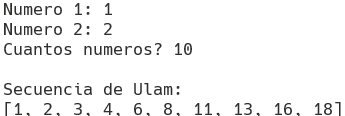
\includegraphics[width=0.8\columnwidth]{12P3.png}
  \end{figure}

  \section*{Conclusiones}
  La utilización de hilos en Java se presenta como un componente crucial para mejorar la multitarea de forma eficaz. Desde la supervisión de los ciclos de vida hasta la coordinación de operaciones, estos hilos representan la solución fundamental para desarrollar aplicaciones que sean ágiles y capaces de adaptarse al crecimiento. Este método, respaldado por las robustas utilidades proporcionadas por Java, permite alcanzar un rendimiento óptimo y gestionar eficientemente los recursos en el complejo contexto de la programación concurrente.

  \twocolumn[
    \centering
    Acosta Porcayo Alan Omar, Gutiérrez Grimaldo Alejandro, Medina Villa Samuel

    \linejump
    
    \textbf{\LARGE{Práctica 13. Patrones de diseño}} \\

    \linejump
  ]

  \footnotetext{
    \scriptsize 
    Acosta Porcayo Alan Omar Ing. en Computación 320206102 \\
    Gutiérrez Grimaldo Alejandro Ing. en Computación 320282098 \\
    Medina Villa Samuel Ing. en Computación 320249538
  }
        
  \fancyfoot{}

  \section*{Resumen}
  La finalidad de la práctica se enfoca en la elaboración de una aplicación en un lenguaje orientado a objetos, integrando el uso de un patrón de diseño específico. Como fase inicial, se llevará a cabo un análisis exhaustivo para comprender diversos patrones de diseño, explorando sus particularidades y aplicaciones. Subsecuentemente, se empleará este conocimiento adquirido durante la creación de la aplicación, seleccionando y aplicando de manera adecuada un patrón de diseño que se adecue a los requisitos del proyecto. Este enfoque no solo aborda la implementación técnica, sino que también destaca la capacidad de tomar decisiones fundamentadas sobre el diseño del software para optimizar la estructura y funcionalidad de la aplicación.

  \section*{Introducción}
  En el ámbito de la ingeniería de software, los patrones de diseño se erigen como soluciones recurrentes y generales para los problemas cotidianos en el diseño de software. Es esencial comprender que un patrón de diseño no constituye un diseño de software completo y listo para la codificación; más bien, se presenta como una descripción o modelo que aborda la resolución de problemas y puede aplicarse en diversas situaciones.

  Los patrones de diseño desempeñan un papel crucial al agilizar el proceso de desarrollo, al proporcionar un paradigma desarrollado y probado. Un diseño de software efectivo debe anticiparse a problemas que pueden surgir durante la implementación, cubriendo exhaustivamente todos los detalles. La reutilización de patrones de diseño emerge como una estrategia para prevenir problemas sutiles y mejorar la legibilidad del código para aquellos familiarizados con los patrones.

  \subsection*{Patrones de Software}
  Cada patrón de diseño aborda problemas recurrentes y presenta soluciones centrales que pueden aplicarse en diversas situaciones. En términos generales, un patrón de diseño consta de cuatro elementos esenciales:

  \begin{enumerate}
    \item \textbf{Nombre del patrón:} Una descripción concisa del diseño del problema y su solución.
    \item \textbf{Problema:} La situación en la que se debe aplicar el patrón, explicando el contexto y, a veces, estableciendo condiciones para su viabilidad.
    \item \textbf{Solución:} La descripción abstracta de los elementos que componen el diseño y cómo resuelven el problema.
    \item \textbf{Consecuencias:} Los resultados y recompensas de aplicar el patrón, críticos para evaluar el diseño alternativo y comprender el impacto en la ingeniería de software.
  \end{enumerate}
  
  Se distinguen tres niveles de patrones de software: arquitectónicos, de diseño y de programación, cada uno abordando diferentes niveles de estructuras de software y hardware.

  \subsection*{Patrón de Diseño Modelo-Vista-Controlador (MVC)}
  El MVC asigna roles a los objetos en la aplicación, definiendo cómo se comunican entre sí. Con capas bien definidas, como el modelo que encapsula la información, la vista que presenta la información y el controlador que actúa como intermediario, el patrón MVC ofrece beneficios en reutilización, claridad de interfaces y facilidad de extensión.

  \begin{itemize}
    \item \textbf{Modelo:} Representa la información y la lógica de manipulación de datos.
    \item \textbf{Vista:} Objeto visible para el usuario, mostrando información y permitiendo la edición.
    \item \textbf{Controlador:} Actúa como intermediario entre vista y modelo, gestionando acciones y el ciclo de vida de los objetos.
  \end{itemize}

  \subsubsection*{Consecuencias del MVC}
  \begin{itemize}
    \item .Desacopla vistas y modelos, estableciendo un protocolo de suscriptor/notificador.
    \item Permite acoplar varias vistas a un modelo y crear nuevas vistas sin modificar el modelo.
    \item Facilita el manejo de entradas del usuario sin alterar la presentación, encapsulando respuestas en el controlador.
  \end{itemize}

  \subsection*{Patrón de Diseño Creacional \textit{Singleton}}
  El \textit{Singleton} aborda la necesidad de una única instancia de una clase, proporcionando control de acceso y reduciendo el espacio de nombres. Permite refinar operaciones y representaciones, así como la flexibilidad de permitir un número variable de instancias.
  
  \subsubsection*{Condiciones para su uso}
  \begin{itemize}
    \item Debe existir exactamente una instancia de una clase accesible desde un punto conocido.
    \item Cuando una única instancia deba existir para una subclase y los clientes utilicen la subclase sin modificar su código.
  \end{itemize}

  \subsection*{Patrón de Diseño Estructural \textit{Composite}}
  El patrón \textit{Composite} define una jerarquía de clases compuestas por objetos primitivos y compuestos. Permite tratar con estructuras compuestas u objetos de manera uniforme, facilita la creación de nuevas funcionalidades y propicia la reutilización.

  \subsubsection*{Consecuencias del \textit{Composite}}
  \begin{itemize}
    \item Define una jerarquía de clases con objetos primitivos y compuestos.
    \item Simplifica la tarea del cliente al tratar con estructuras compuestas de manera uniforme.
    \item Facilita la creación de nuevas funcionalidades y puede hacer difícil restringir componentes nuevos debido a su facilidad de adición.
  \end{itemize}

  \subsection*{Patrón de Diseño de Comportamiento \textit{Observer}}
  Este patrón aborda la necesidad de notificar a un grupo de objetos sobre un evento en la aplicación. Al dividir el sistema en clases cooperativas, el \textit{Observer} garantiza consistencia de información entre objetos relacionados, permitiendo un bajo acoplamiento y reutilización.

  \textbf{Problema:} Notificar a diferentes objetos sobre un evento en la aplicación, sin saber cuántos objetos deben reflejar el cambio.

  \textbf{Solución:} Crear una clase abstracta que maneje un conjunto de objetos observadores. Cuando cambie el sujeto observado, notificar a todos los observadores.

  \subsubsection*{Consecuencias del \textit{Observer}}
  \begin{itemize}
    \item Parte el sistema en clases cooperativas para consistencia de información.
    \item Permite un bajo acoplamiento y reutilización de clases.
  \end{itemize}

  \section*{Objetivos}
  \begin{itemize}
    \item Aplicar un patrón de diseño específico para mejorar la eficiencia y el rendimiento de la aplicación
    \item Implementar patrones que mejoren la gestión de errores y excepciones en la aplicación
    \item Implementar una aplicación en un lenguaje orientado a objetos utilizando algún patrón de diseño.
  \end{itemize}

  \section*{Resultados}
  \subsection*{Problema 1}
  Usando el patrón creacional \textit{Singleton} programe ``el genio de la lampará''. El genio solo puede ser usado por una persona y el genio solo puede usada como una y sólo una instancia. El genio pregunta tres deseos de una persona y los cumple.

  \textit{\textbf{Solución}}
  \begin{lstlisting}
import java.util.Scanner;

class Genio {
  private static Genio instancia;
  public String nombre;

  private Genio(String nombre) {
    this.nombre = nombre;
  }

  public static Genio getInstancia(String nombre) {
    if (instancia == null)
      instancia = new Genio(nombre);

    return instancia;
  }

  public void pedirDeseo() {
    Scanner sc = new Scanner(System.in);
    
    System.out.print("Cual es tu deseo?\n> ");
    String deseo = sc.nextLine();

    System.out.println("Pensando...");

    try {
      Thread.sleep(3000);
    } catch (InterruptedException e) {
      e.printStackTrace();
    }

    System.out.println("Tu deseo se ha cumplido!!!\n");

    sc.close();
  }
}

public class Problema1 {
  public static void main(String[] args) {
    Genio genio = Genio.getInstancia("Genio");

    genio.pedirDeseo();
    genio.pedirDeseo();
    genio.pedirDeseo();
  }
}
  \end{lstlisting}

  \textbf{Ejecución}
  \begin{figure}[h!]
    \centering
    
\includegraphics[width=0.6\columnwidth]{13P1.png}
  \end{figure}

  \subsection*{Problema 2}
  Implementa el patrón de diseño de estructura \textit{Bridge} que se describe en el problema de figuras y colores en: \url{https://refactoring.guru/design-patterns/bridge}

  Considere 2 figuras y 2 colores adicionales al problema.

  \begin{figure}[h!]
    \centering
    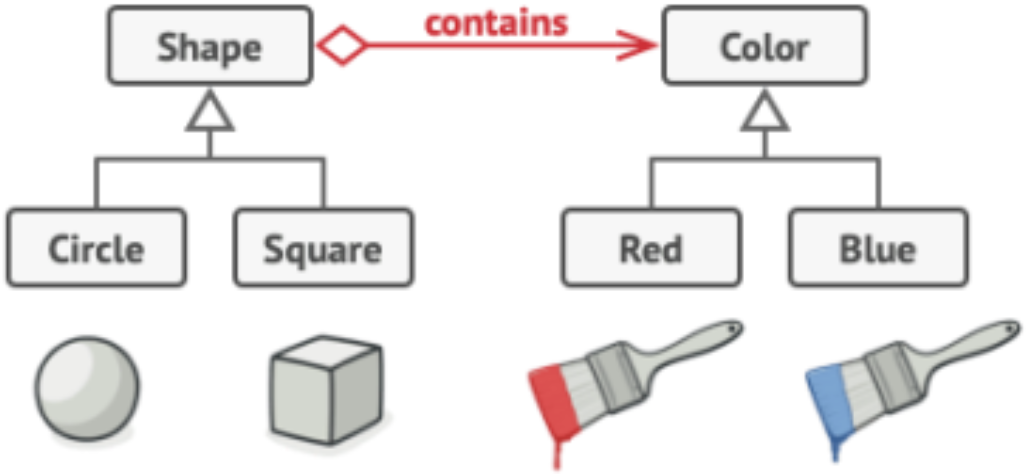
\includegraphics[width=\columnwidth]{bridge.png}
  \end{figure}

  \textit{\textbf{Shape.java}}
  \begin{lstlisting}
public class Shape {
  Color color;
  String nombre;

  public Shape(Color color, String nombre) {
    this.color = color;
    this.nombre = nombre;
  }

  @Override
  public String toString() {
    return "Nombre: " + nombre + "\tColor: " + color;
  }
}

class Circle extends Shape {
  public Circle(Color color, String nombre) {
    super(color, nombre);
  }
}

class Rectangle extends Shape {
  public Rectangle(Color color, String nombre) {
    super(color, nombre);
  }
}

class Triangle extends Shape {
  public Triangle(Color color, String nombre) {
    super(color, nombre);
  }
}

class Square extends Shape {
  public Square(Color color, String nombre) {
    super(color, nombre);
  }
}
  \end{lstlisting}

  \textit{\textbf{Color.java}}
  \begin{lstlisting}
public class Color {
  String tipo;
  
  public String toString() {
    return tipo;
  }
}

class Red extends Color {
  public Red () {
    tipo = "Rojo";
  }
}

class Blue extends Color {
  public Blue () {
    tipo = "Azul";
  }
}

class Green extends Color {
  public Green () {
    tipo = "Verde";
  }
}

class Yellow extends Color {
  public Yellow () {
    tipo = "Amarillo";
  }
}
  \end{lstlisting}

  \textit{\textbf{Problema2.java}}
  \begin{lstlisting}
public class Problema2 {
  public static void main(String[] args) {
    Circle circulo = new Circle(new Red(), "Circulo 1");
    Rectangle rectangulo = new Rectangle(new Blue(), "Rectangulo 1");
    Triangle triangulo = new Triangle(new Green(), "Triangulo 1");
    Square cuadrado = new Square(new Yellow(), "Cuadrado 1");

    System.out.println(circulo);
    System.out.println(rectangulo);
    System.out.println(triangulo);
    System.out.println(cuadrado);
  }
}
  \end{lstlisting}

  \textbf{Ejecución}
  \begin{figure}[h!]
    \centering
    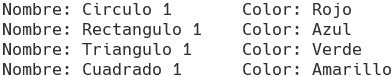
\includegraphics[width=0.75\columnwidth]{13P2.png}
  \end{figure}

  \section*{Conclusiones}
  Los patrones de diseño en el ámbito de la ingeniería de software proporcionan soluciones comprobadas y recurrentes para enfrentar desafíos típicos en el diseño de aplicaciones. Desde la mejora del rendimiento hasta asegurar la adaptabilidad y mantenibilidad del código, la aplicación efectiva de estos patrones posibilita la construcción de sistemas resistentes y flexibles. Al entender y emplear de manera adecuada patrones creacionales, estructurales y de comportamiento, los desarrolladores tienen la capacidad de perfeccionar la eficiencia, seguridad y usabilidad de sus aplicaciones, lo que a su vez contribuye a un desarrollo de software más eficaz y sostenible.

  \section*{Referencias}
  \begin{small}
    \textit{Bridge.} (2014). Refactoring.guru. \url{https://refactoring.guru/design-patterns/bridge} \\

    Solano, J. (2017, 20 enero). \textit{Manual de prácticas de Programación Orientada a Objetos}. Laboratorio de Computación Salas A y B. \url{http://lcp02.fi-b.unam.mx/} \\
  \end{small}
\end{document}